\documentclass[serif,mathserif,final]{beamer}
\usepackage{epsf}
\usepackage{subfigure}
\usepackage{tabularx}
\usepackage{subfigure}
\usepackage{graphicx}
\usepackage{wrapfig}
\usepackage{url}
\usepackage{tikz}
\usepackage{color}
\usepackage{epstopdf}
\usepackage{algorithm}
\usepackage{algorithmic}
\usepackage{eqparbox}
\usepackage{epstopdf}
\usepackage{textcomp}
\usepackage{tabulary}
\usepackage{multirow}
\usepackage{latexsym}
\usepackage{amsmath,amsfonts,amssymb,xspace}
\usepackage{graphicx}

\renewcommand{\algorithmiccomment}[1]{\hfill\eqparbox{COMMENT}{#1}}
\setbeamertemplate{bibliography item}[text]
\setbeamertemplate{bibliography entry title}{}
\setbeamertemplate{bibliography entry location}{}
\setbeamertemplate{bibliography entry note}{}
\mode<presentation>{
\definecolor{uagreen}{RGB}{0,124,65}
\definecolor{utor}{RGB}{12,28,71}
\definecolor{utor2}{RGB}{0,32,78}
\setbeamercolor{structure}{fg=utor2}
\setbeamercolor{headline}{bg=white}
\setbeamercolor{footline}{bg=black}
\setbeamerfont{footline}{size=\large}
\setbeamercolor{separation line}{bg=black}
\setbeamercolor{title in headline}{fg=utor2}
\setbeamercolor{author in headline}{fg=black}
\setbeamercolor{institute in headline}{fg=lightgray}
\setbeamercolor{framesubtitle}{fg=blue, bg=gray}
\setbeamercolor{author in head/foot}{fg=black,bg=black}
%\setbeamercolor{title in head/foot}{fg=butter,bg=black}
%\setbeamercolor{website in footline}{fg=butter,bg=black}
%\setbeamercolor{email in footline}{fg=butter,bg=black}
\setbeamercolor{section in head/foot}{use=structure,bg=structure.fg!25!bg}
\setbeamertemplate{headline}{%
\leavevmode
{\usebeamercolor{section in head/foot}}
\pgfdeclareverticalshading{beamer@headfade}{\paperwidth}{%
color(0cm)=(bg); color(1.5cm)=(section in head/foot.bg) }
\setbeamercolor{section in head/foot}{bg=} 
\begin{beamercolorbox}[wd=\paperwidth]{headline}
  \begin{columns}[T]
    \begin{column}{.04\paperwidth} %0.02
    \end{column}
    \begin{column}{0.05\paperwidth} %0.07
      \centering
      \vskip4ex
      \vspace{1pt}
    \end{column}
    \begin{column}{.675\paperwidth} %0.675
      \vskip4ex
      \usebeamercolor{title in headline}
      {\color{fg}\textbf{\LARGE{\inserttitle}}\\[1ex]}
      \usebeamercolor{author in headline}
      {\color{fg}\Large{\insertauthor} \hspace{15mm}}
      \usebeamercolor{institute in headline}
      {\color{fg}\large{\insertinstitute}\\[1ex]}
      \vskip2ex
      \end{column}
      \begin{column}{.25\paperwidth}
        \centering
        \vskip4ex
        \hspace{-2in}
        
\includegraphics[height=0.04\paperwidth]{logo.jpg} %0.025
        \vspace{1pt}
      \end{column}
      \begin{column}{.03\paperwidth}
      \end{column}
    \end{columns}
  \end{beamercolorbox}

  \begin{beamercolorbox}[wd=\paperwidth]{lower separation line head}
    \rule{0pt}{2pt}
  \end{beamercolorbox} 
}

%\addtoheadtemplate{\pgfuseshading{beamer@headfade}\vskip-1.5cm}{}
\setbeamertemplate{items}[ball]   % 3-D balls for itemize/enumerate
%\useoutertheme{umbcfootline}
\mode<all>
}

\graphicspath{{./figures/}} %142.24, 96.52
\usepackage[orientation=landscape,
size=custom,width=111.76,height=96.52,scale=1.4,debug]{beamerposter} %0.6
%\usepackage[orientation=landscape,scale=1.25,debug]{beamerposter}

%-- Header and footer information ----------------------------------
%\newcommand{\footleft}{http://www.shawnlankton.com/category/latex/}
%\newcommand{\footright}{shawn at shawn lankton dot com}
\title{\huge{Exploring Models and Data for Image Question Answering}}
\author{Mengye Ren, Ryan Kiros, Richard S. Zemel}
\institute{University of Toronto}
%-------------------------------------------------------------------

%-- Main Document --------------------------------------------------
\begin{document}
\begin{frame}{}
\begin{columns}[t]

%-- Column 1 ---------------------------------------------------
\begin{column}{0.32\linewidth}
\minipage[c][0.9\textheight][s]{\columnwidth}
\vfill

%-- Block 1-1 --------------------------------------------------
\begin{block}{\bf{\large The problems to solve}}
	\begin{itemize}
	  \item Retrieve and generate descriptions of images
	\end{itemize}
  \begin{figure}[t!]
    \vspace{-0.1in}
    \centering
    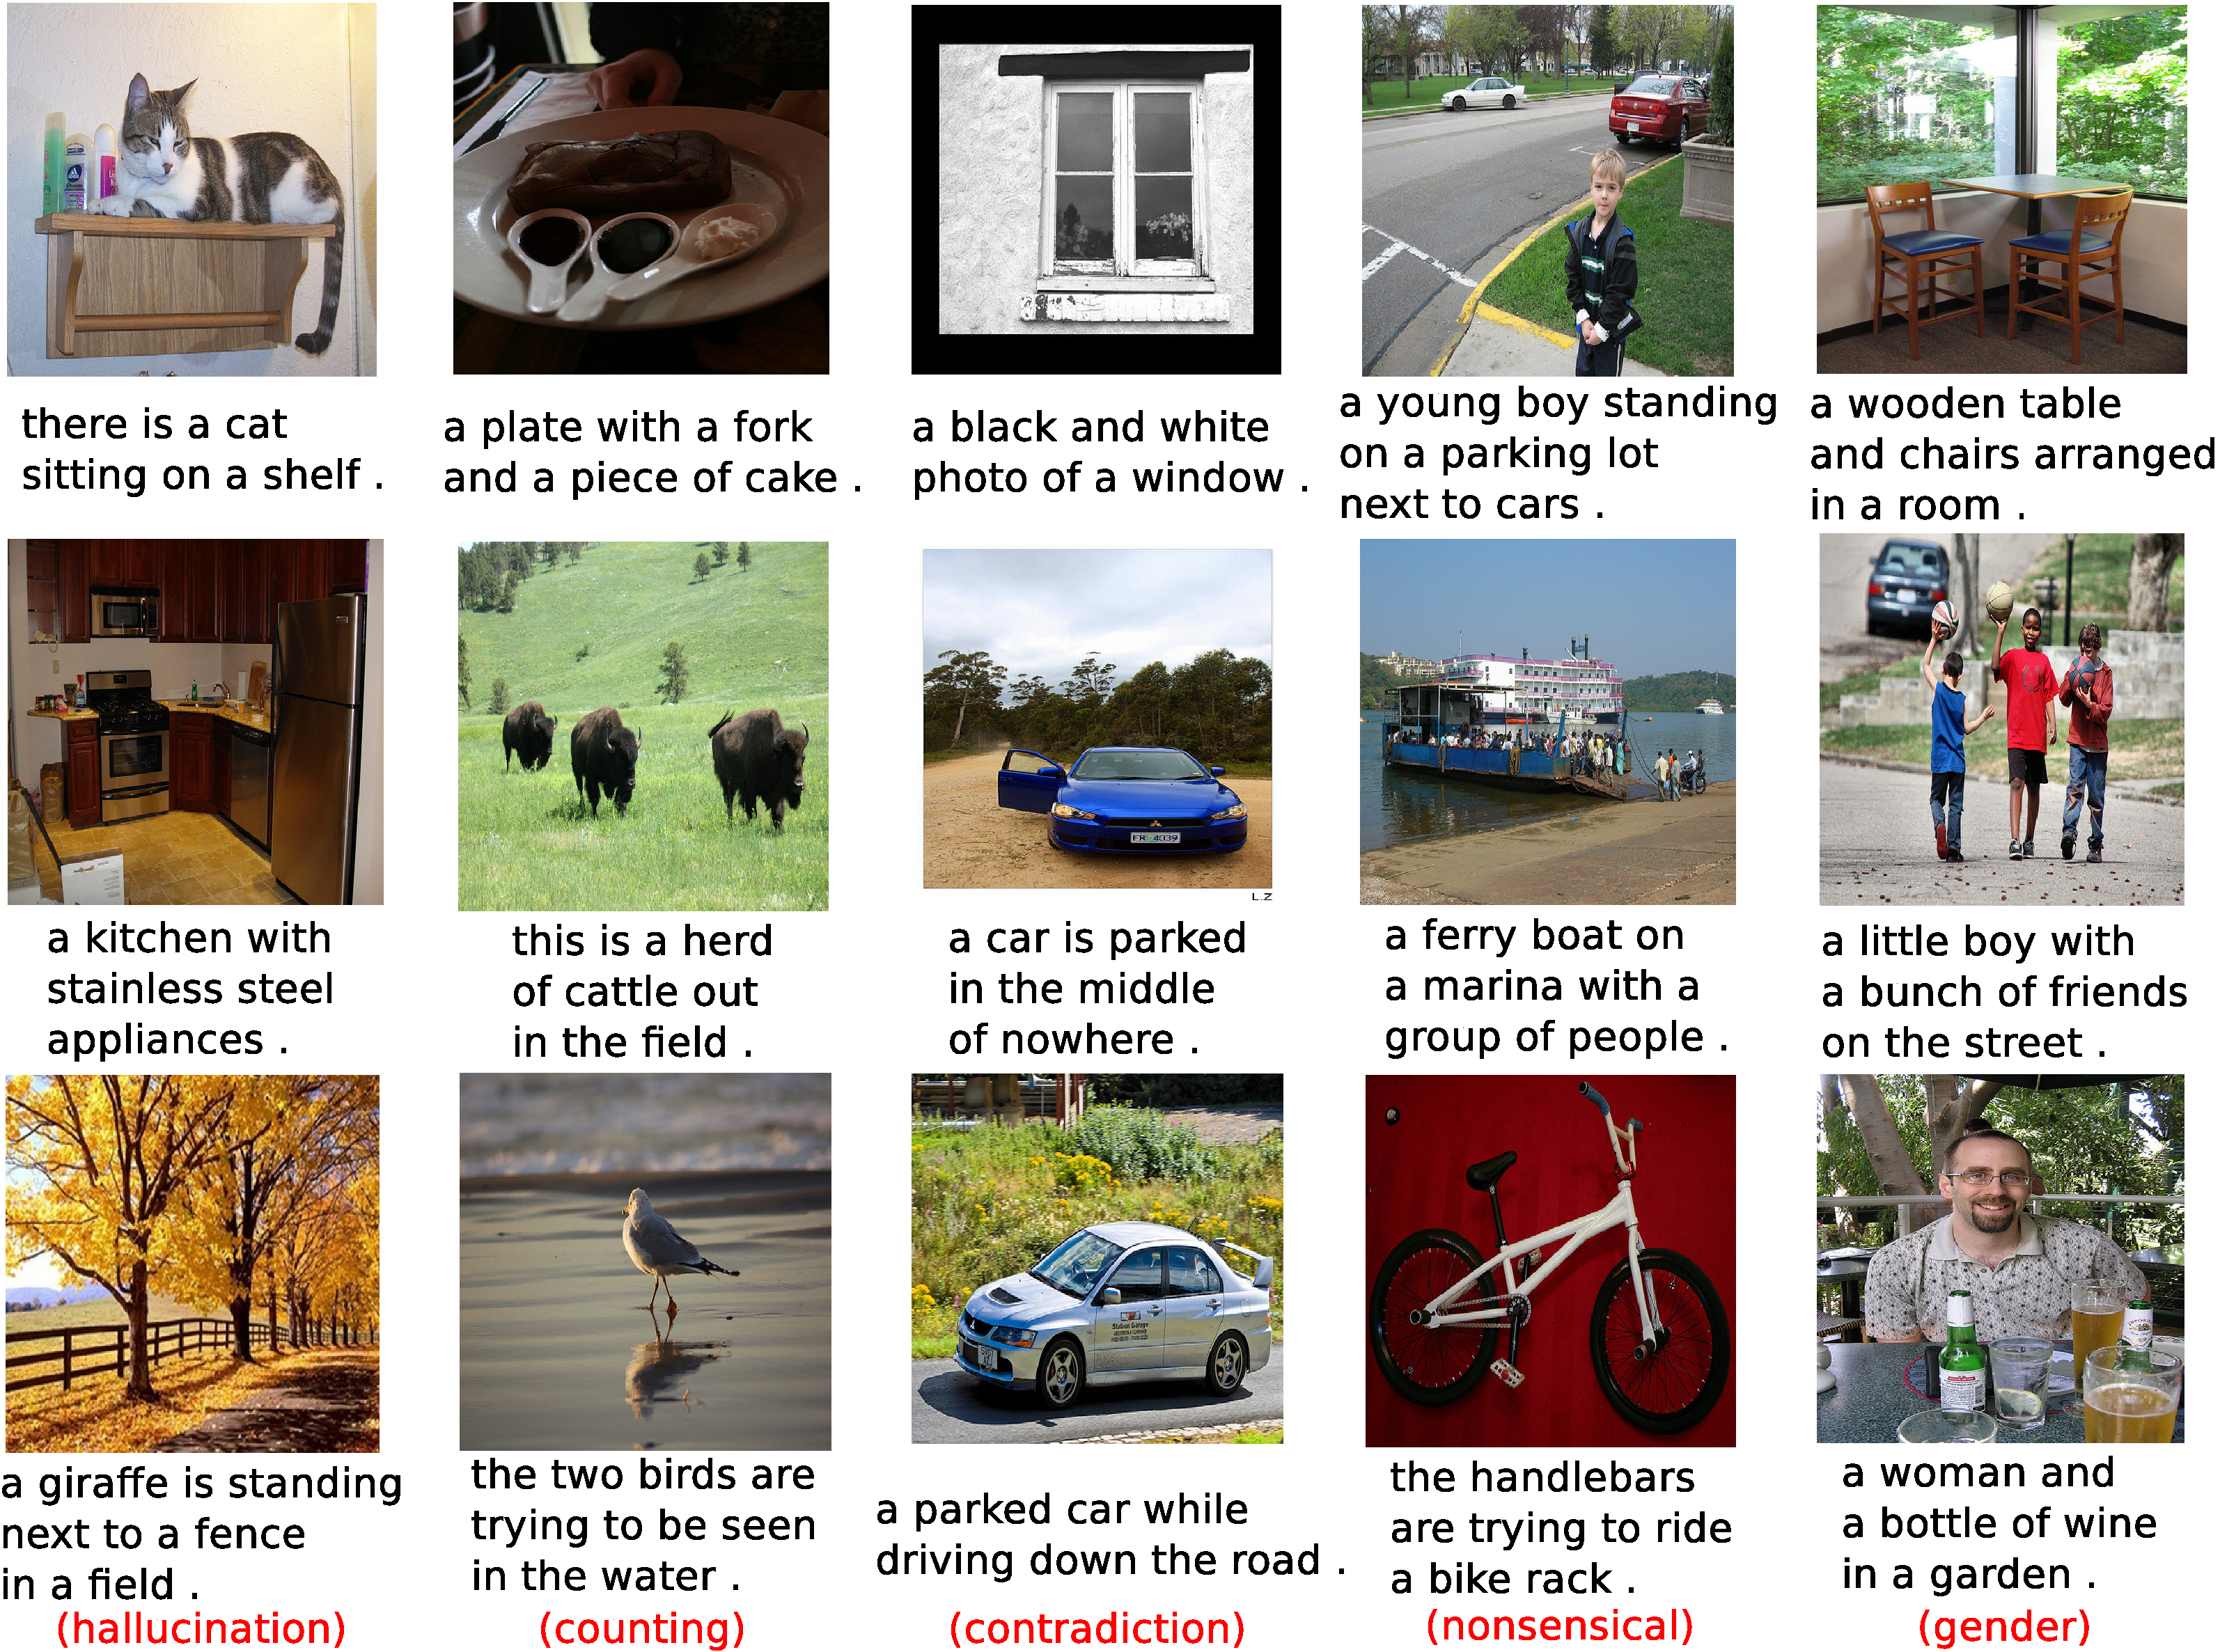
\includegraphics[width=0.85\columnwidth]{caption_results.pdf}
    \vspace{-0.1in}
    \caption{Sample generated captions from our proposed model.
    The bottom row shows some representative error cases, along with our
    description (in red) of the type of error. None of these generated
    descriptions appear word for word in the training set.} 
    \label{fig:annot}
  \end{figure}
\end{block}
\vfill

%-- Block 1-2 --------------------------------------------------
\begin{block}{\bf{\large Our encoder-decoder model}}
  \begin{itemize}
  \item Encoder-decoder model
  \end{itemize}
  \begin{figure}[t!]
    \centering
    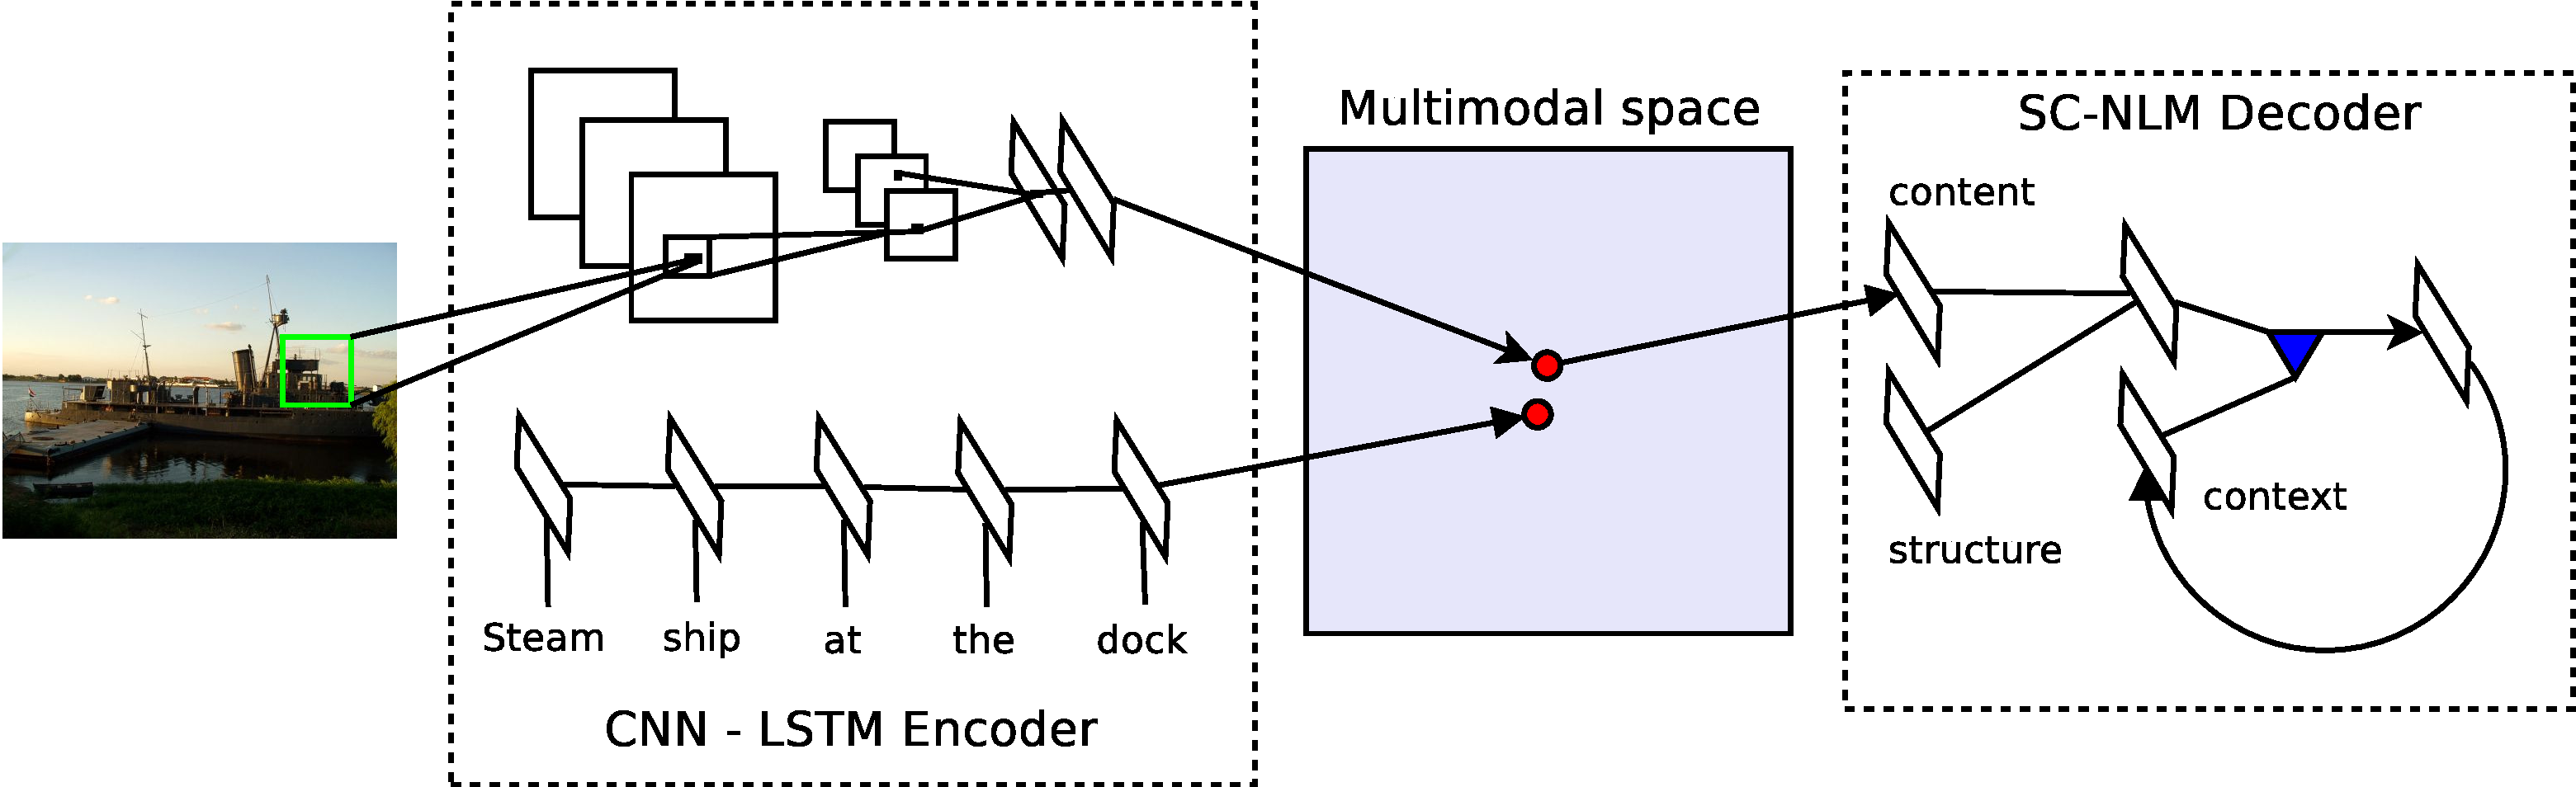
\includegraphics[width=0.9\columnwidth]{encdec2}
    \caption{\textbf{Encoder:} A deep convolutional network (CNN) and long
      short-term memory recurrent network (LSTM) for learning a joint
      image-sentence embedding. \textbf{Decoder:} A new neural language model that
      combines structure and content vectors for generating words one at a time in
      sequence.} 
    \label{fig:annot2}
  \end{figure}
\end{block}
\vfill

%-- Block 1-3 --------------------------------------------------
\begin{block}{\bf{\large Encoder (ConvNet-LSTM)}}  
  \begin{itemize}
    \item Given: (image, sentence) training pairs           
    \begin{figure}[t!]
      \vspace{-0.1in}
      \centering
      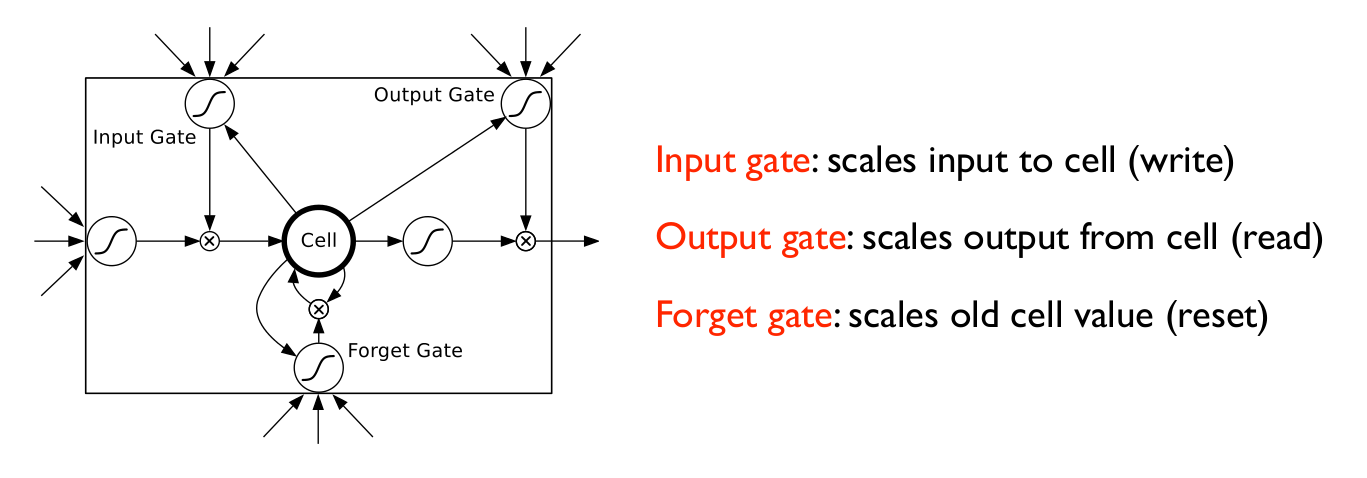
\includegraphics[width=0.9\columnwidth]{lstm}
      \vspace{-0.1in}
      \caption{LSTM. Inputs are word vectors, hidden states gives sentence vectors.} 
      \label{fig:annot}
    \end{figure}
    \item ${\bf x}$: linear transformation of ConvNet 4096 dim output, unit norm
    \item ${\bf v}$: Sentence embedding (hidden state of the LSTM), unit norm
    \item Minimize the following pairwise ranking loss:
    \begin{eqnarray}
    \small
    \underset{\boldsymbol\theta}{\operatorname{min}} \hspace{1mm}
    \label{eq:rank}
    \sum_{\bf x} \sum_k \text{max}\{0, \alpha - s({\bf x}, {\bf v}) + s({\bf x}, {\bf v}_k)\} 
    + \sum_{\bf v} \sum_k \text{max}\{0, \alpha - s({\bf v}, {\bf x}) + s({\bf v}, {\bf x}_k)\}, 
    \nonumber 
    \end{eqnarray}
    \item Where ${\bf v}_k, {\bf x}_k$ are contrastive terms
  \end{itemize}
\end{block}
\vfill
\endminipage
\end{column}

%-- Column 2 ---------------------------------------------------
\begin{column}{0.32\linewidth}

\minipage[c][0.9\textheight][s]{\columnwidth}

%-- Block 2-1 --------------------------------------------------
\vfill
\begin{block}{\bf{\large Decoder (SC-NLM)}}  
  \begin{itemize}
  \item Let ${\bf v}$ denote the image embedding from the multimodal space
  \item Given a sentence $w_1, \ldots, w_N$, 
    with corresponding POS tags $t_1, \ldots, t_N$
  \item Model the distribution $P(w_n = i | w_{1:n-1}, t_{n:n+k}, 
  {\bf v})$ for previous word context $w_{1:n-1}$ 
  and forward POS context $t_{n:n+k}$
  \end{itemize}
  \begin{figure}
    \centering
    \mbox{
      \subfigure[Multiplicative NLM]
      {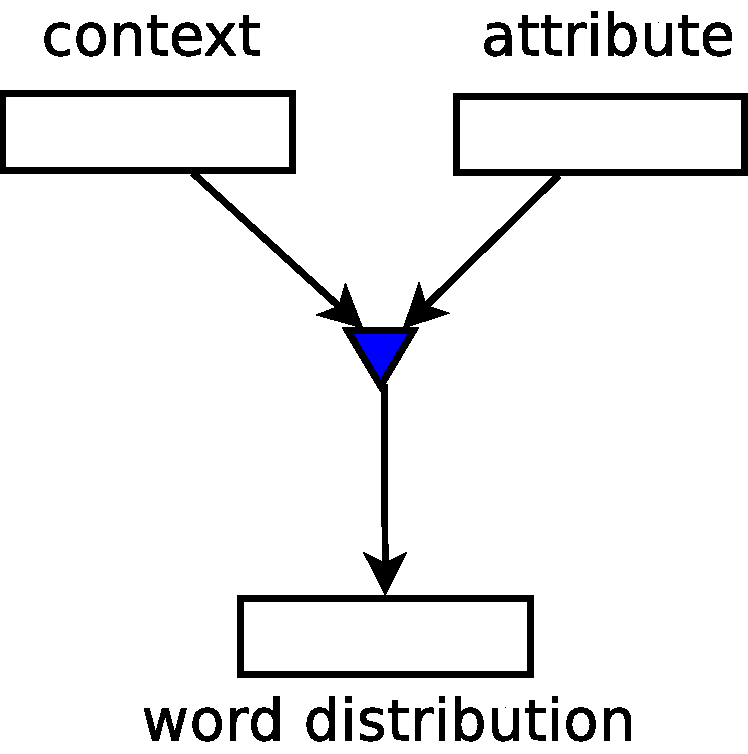
\includegraphics[width=0.29\columnwidth]{l2.pdf}}%\quad
      \hspace{5mm}
      \subfigure[Structure-content NLM]
      {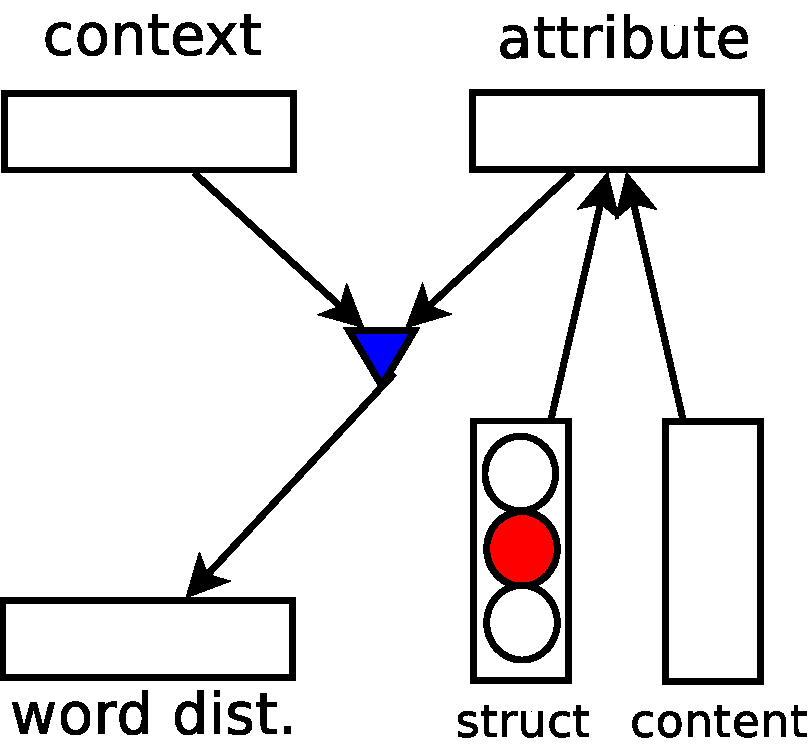
\includegraphics[width=0.316\columnwidth]{l3a.pdf}}\quad
      \hspace{2mm}
      \subfigure[SC-NLM prediction]
      {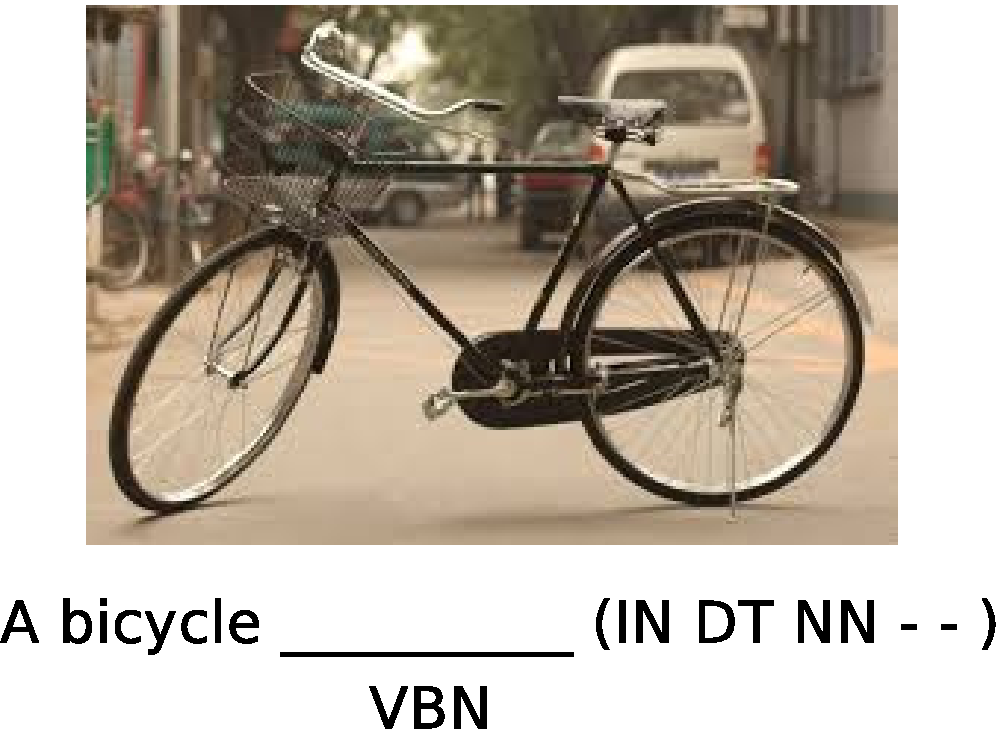
\includegraphics[width=0.33\columnwidth]{stnlm.pdf}}%\quad
    }

    \caption{{\bf Left:} Multiplicative neural language model. {\bf Middle:}
      Structure-content neural language model (SC-NLM). {\bf Right:} The
      prediction problem of an SC-NLM: estimate 
      $P(w_n = i | w_{1:n-1}, t_{n:n+k}, {\bf v})$, where ``A bicycle'' is the context 
      $w_{1:n-1}$, ``VBN IN DT NN'' is the forward structure context
      $t_{n:n+k}$, and the content ${\bf v}$ is the image embedding.}
    \label{fig:nlms}
  \end{figure}
\end{block}
\vfill

%-- Block 2-2--------------------------------------------------
\begin{block}{\bf{\large How to generate descriptions}} 
  \begin{itemize}
  \item Given an image, map it into the multimodal space to get ${\bf v}$
  \item Sample a POS sequence from the training set
  \item Generate a description ${\bf x}$ from the SC-NLM
  \item Score the description with a \textbf{translation model} $(s({\bf x}, {\bf v}))$ and an n-gram \textbf{language model}.
  \end{itemize}
\end{block}
\vfill

%-- Block 2-3 --------------------------------------------------
\begin{block}{\bf{\large Experiment: Localization}}  
  \begin{itemize}
  \item How well can we localize objects after training?
  \end{itemize}
  \begin{figure}
    \centering
    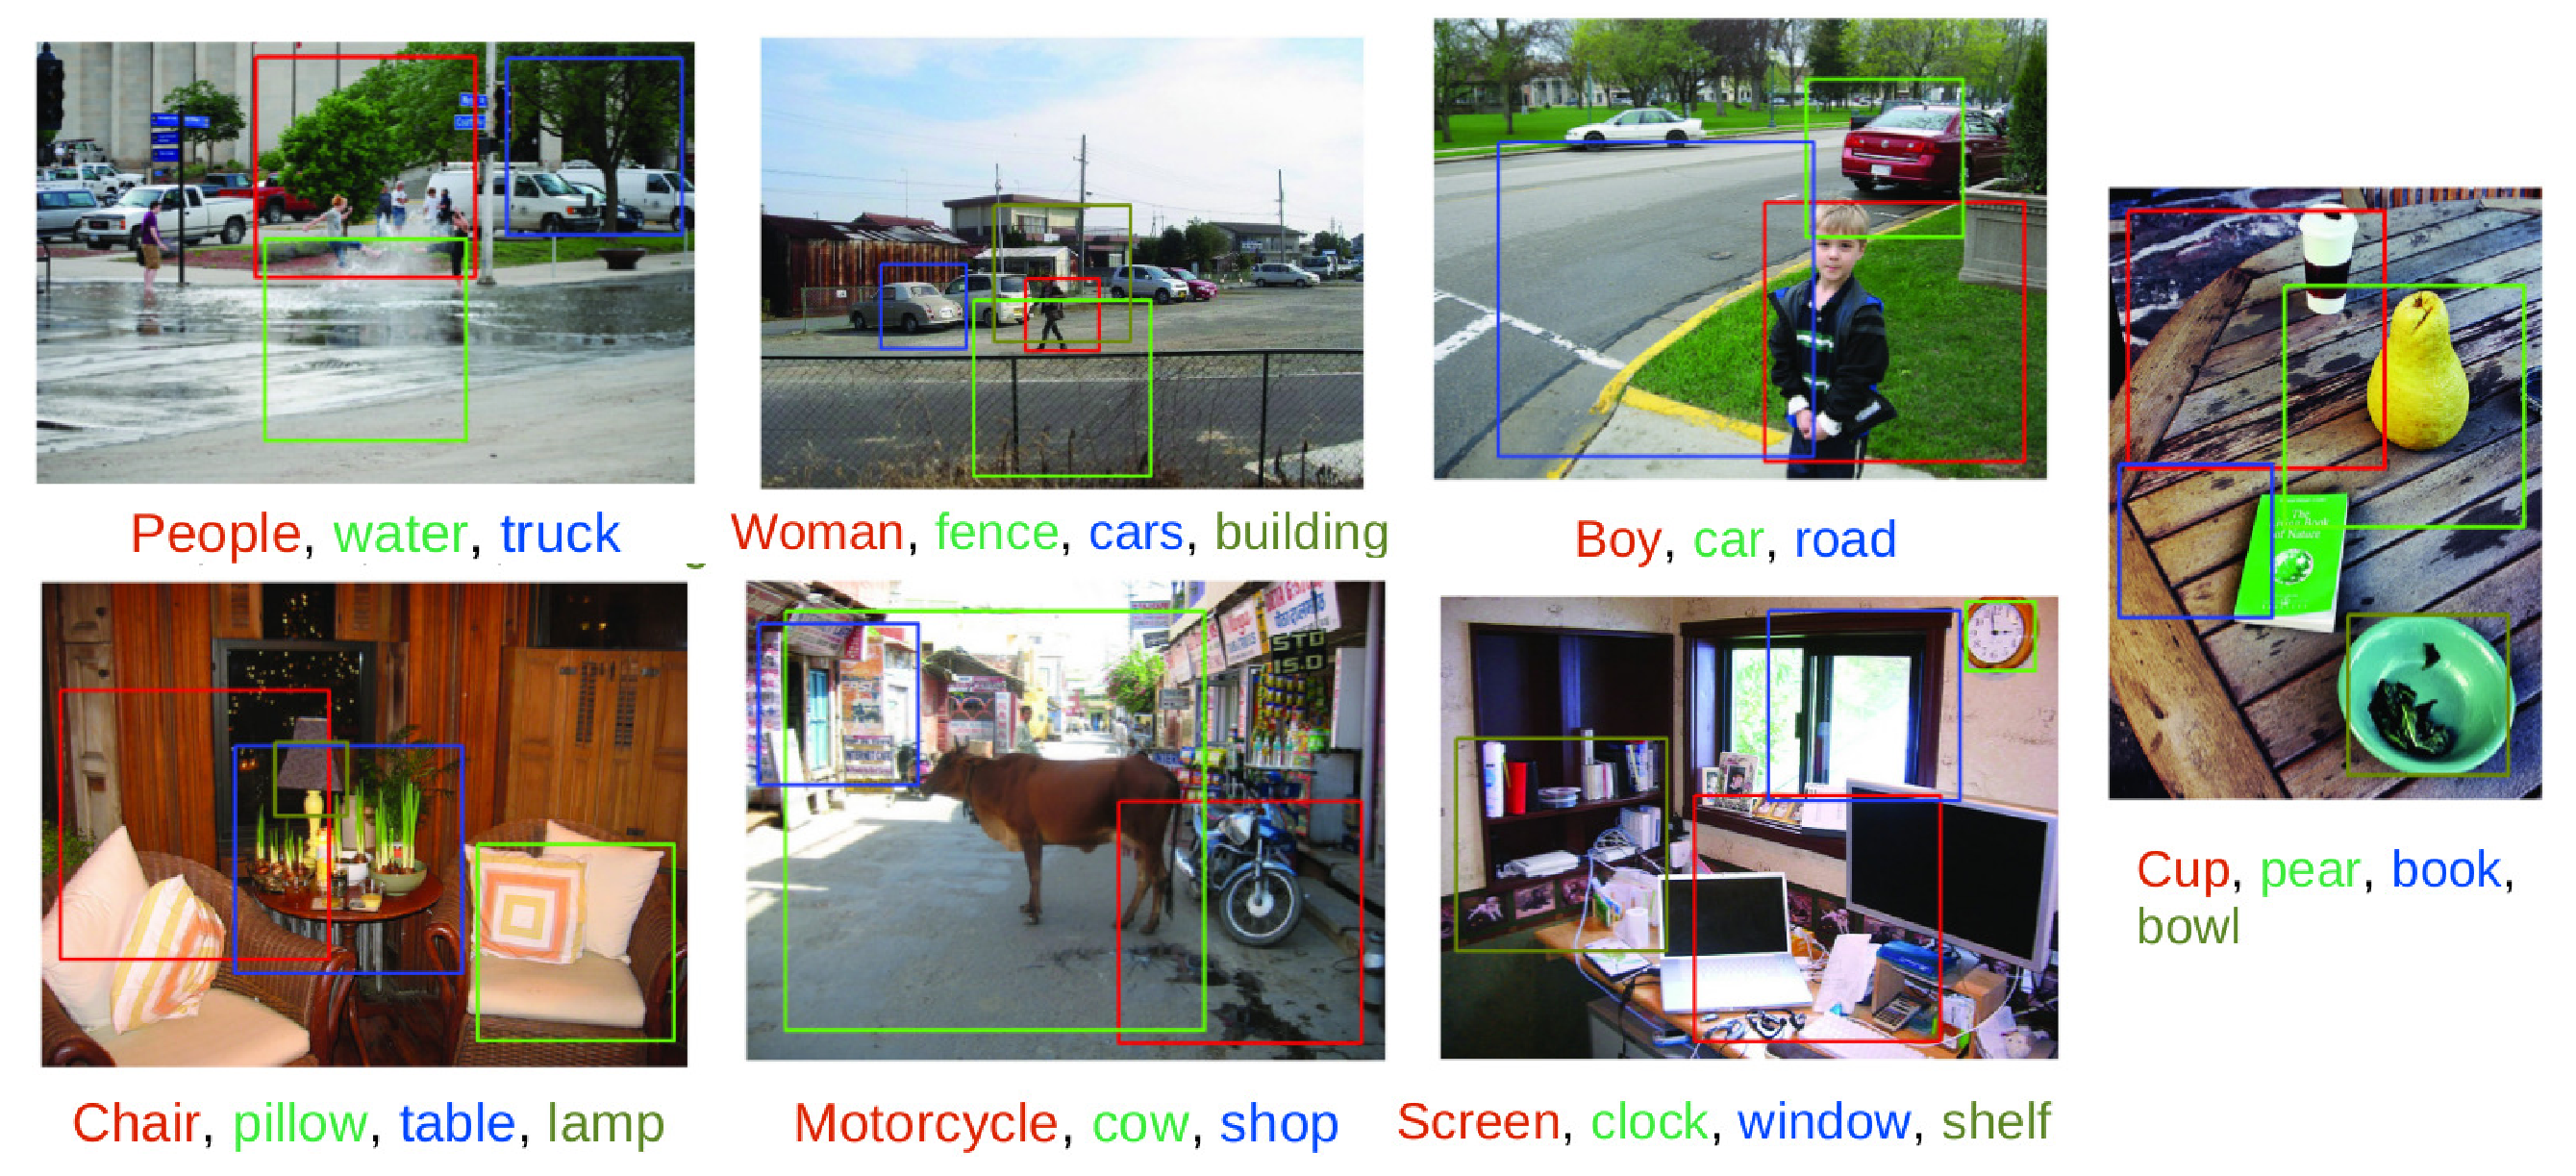
\includegraphics[width=0.9\columnwidth]{align} 
    \caption{Self-taught object localization. Even though our model does not
      incorporate object detections during training, it can still learn to
      localize.}
    \label{fig:local}
  \end{figure}
\end{block}
\vfill   

%-- Block 2-4 --------------------------------------------------
\begin{block}{\bf{\large Experiment: Multimodal linguistic regularities}}  
  \begin{itemize}
  \item Multimodal vector space arithmetic with a linear encoder
  \end{itemize}
  \begin{figure}
    \centering
    \mbox{
      \subfigure[Colors]
      {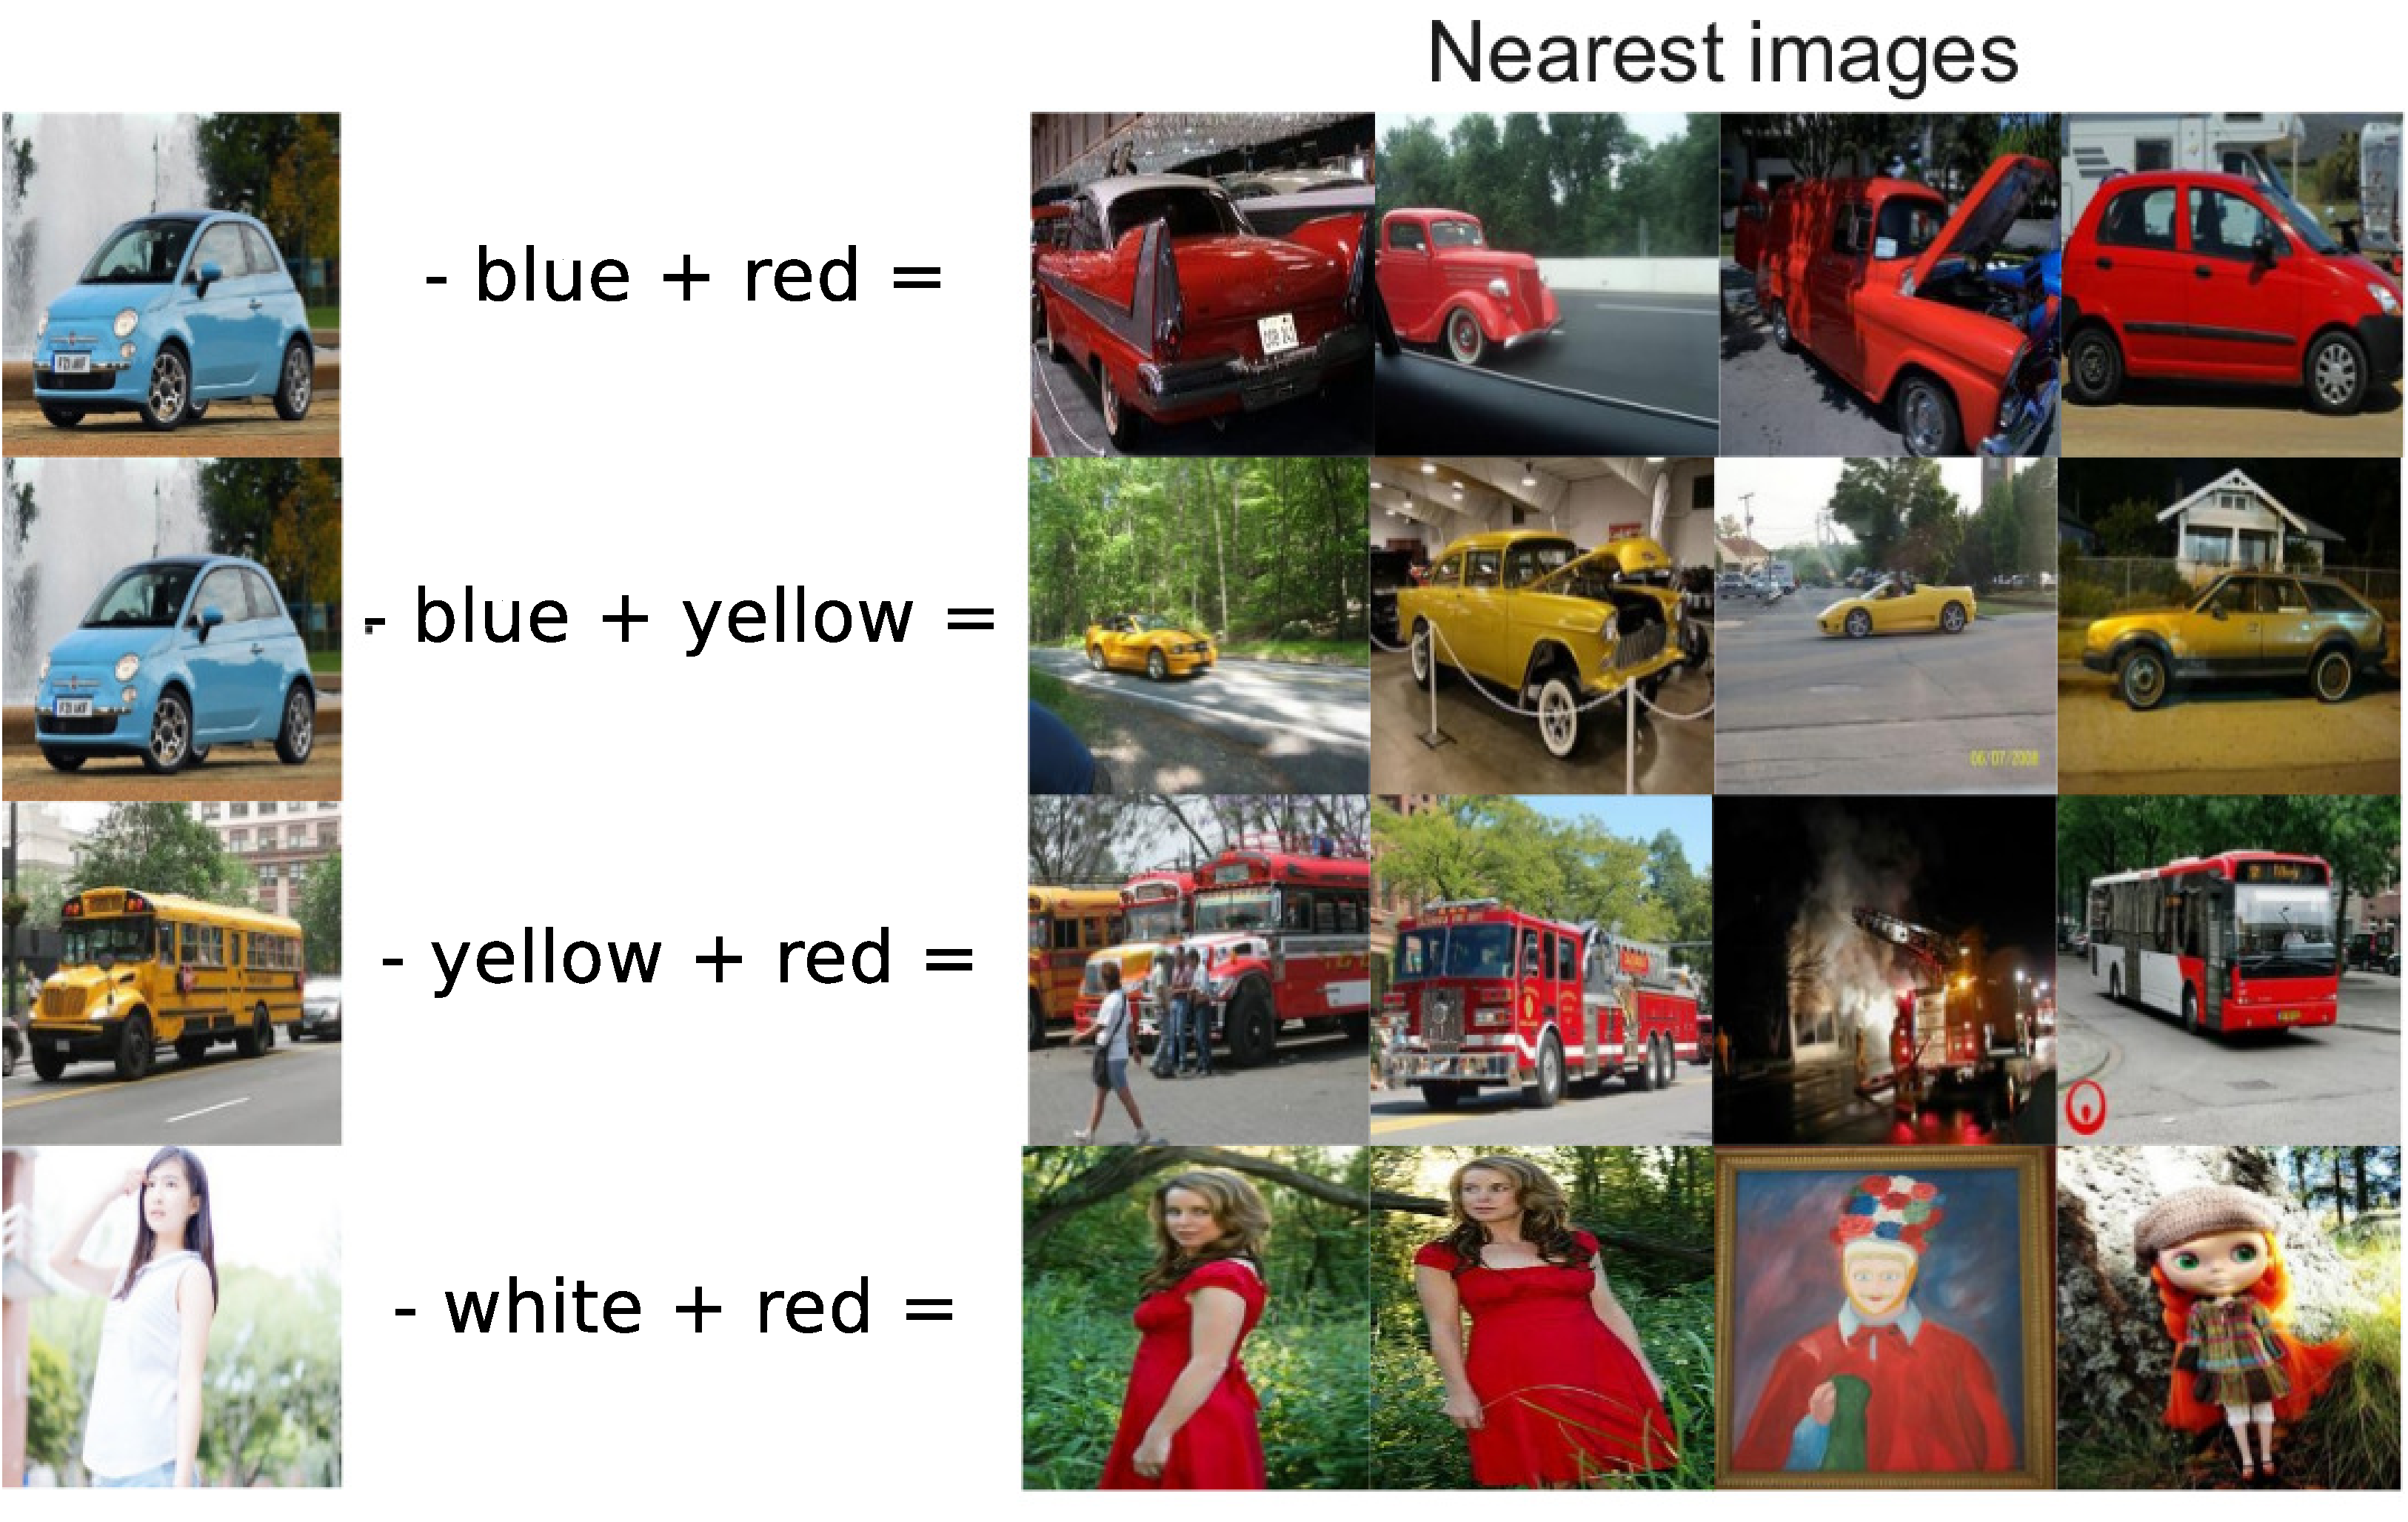
\includegraphics[width=0.33\columnwidth]{colors_crop2.pdf}}
      \hspace{0.1in}
      \subfigure[Image structure]
      {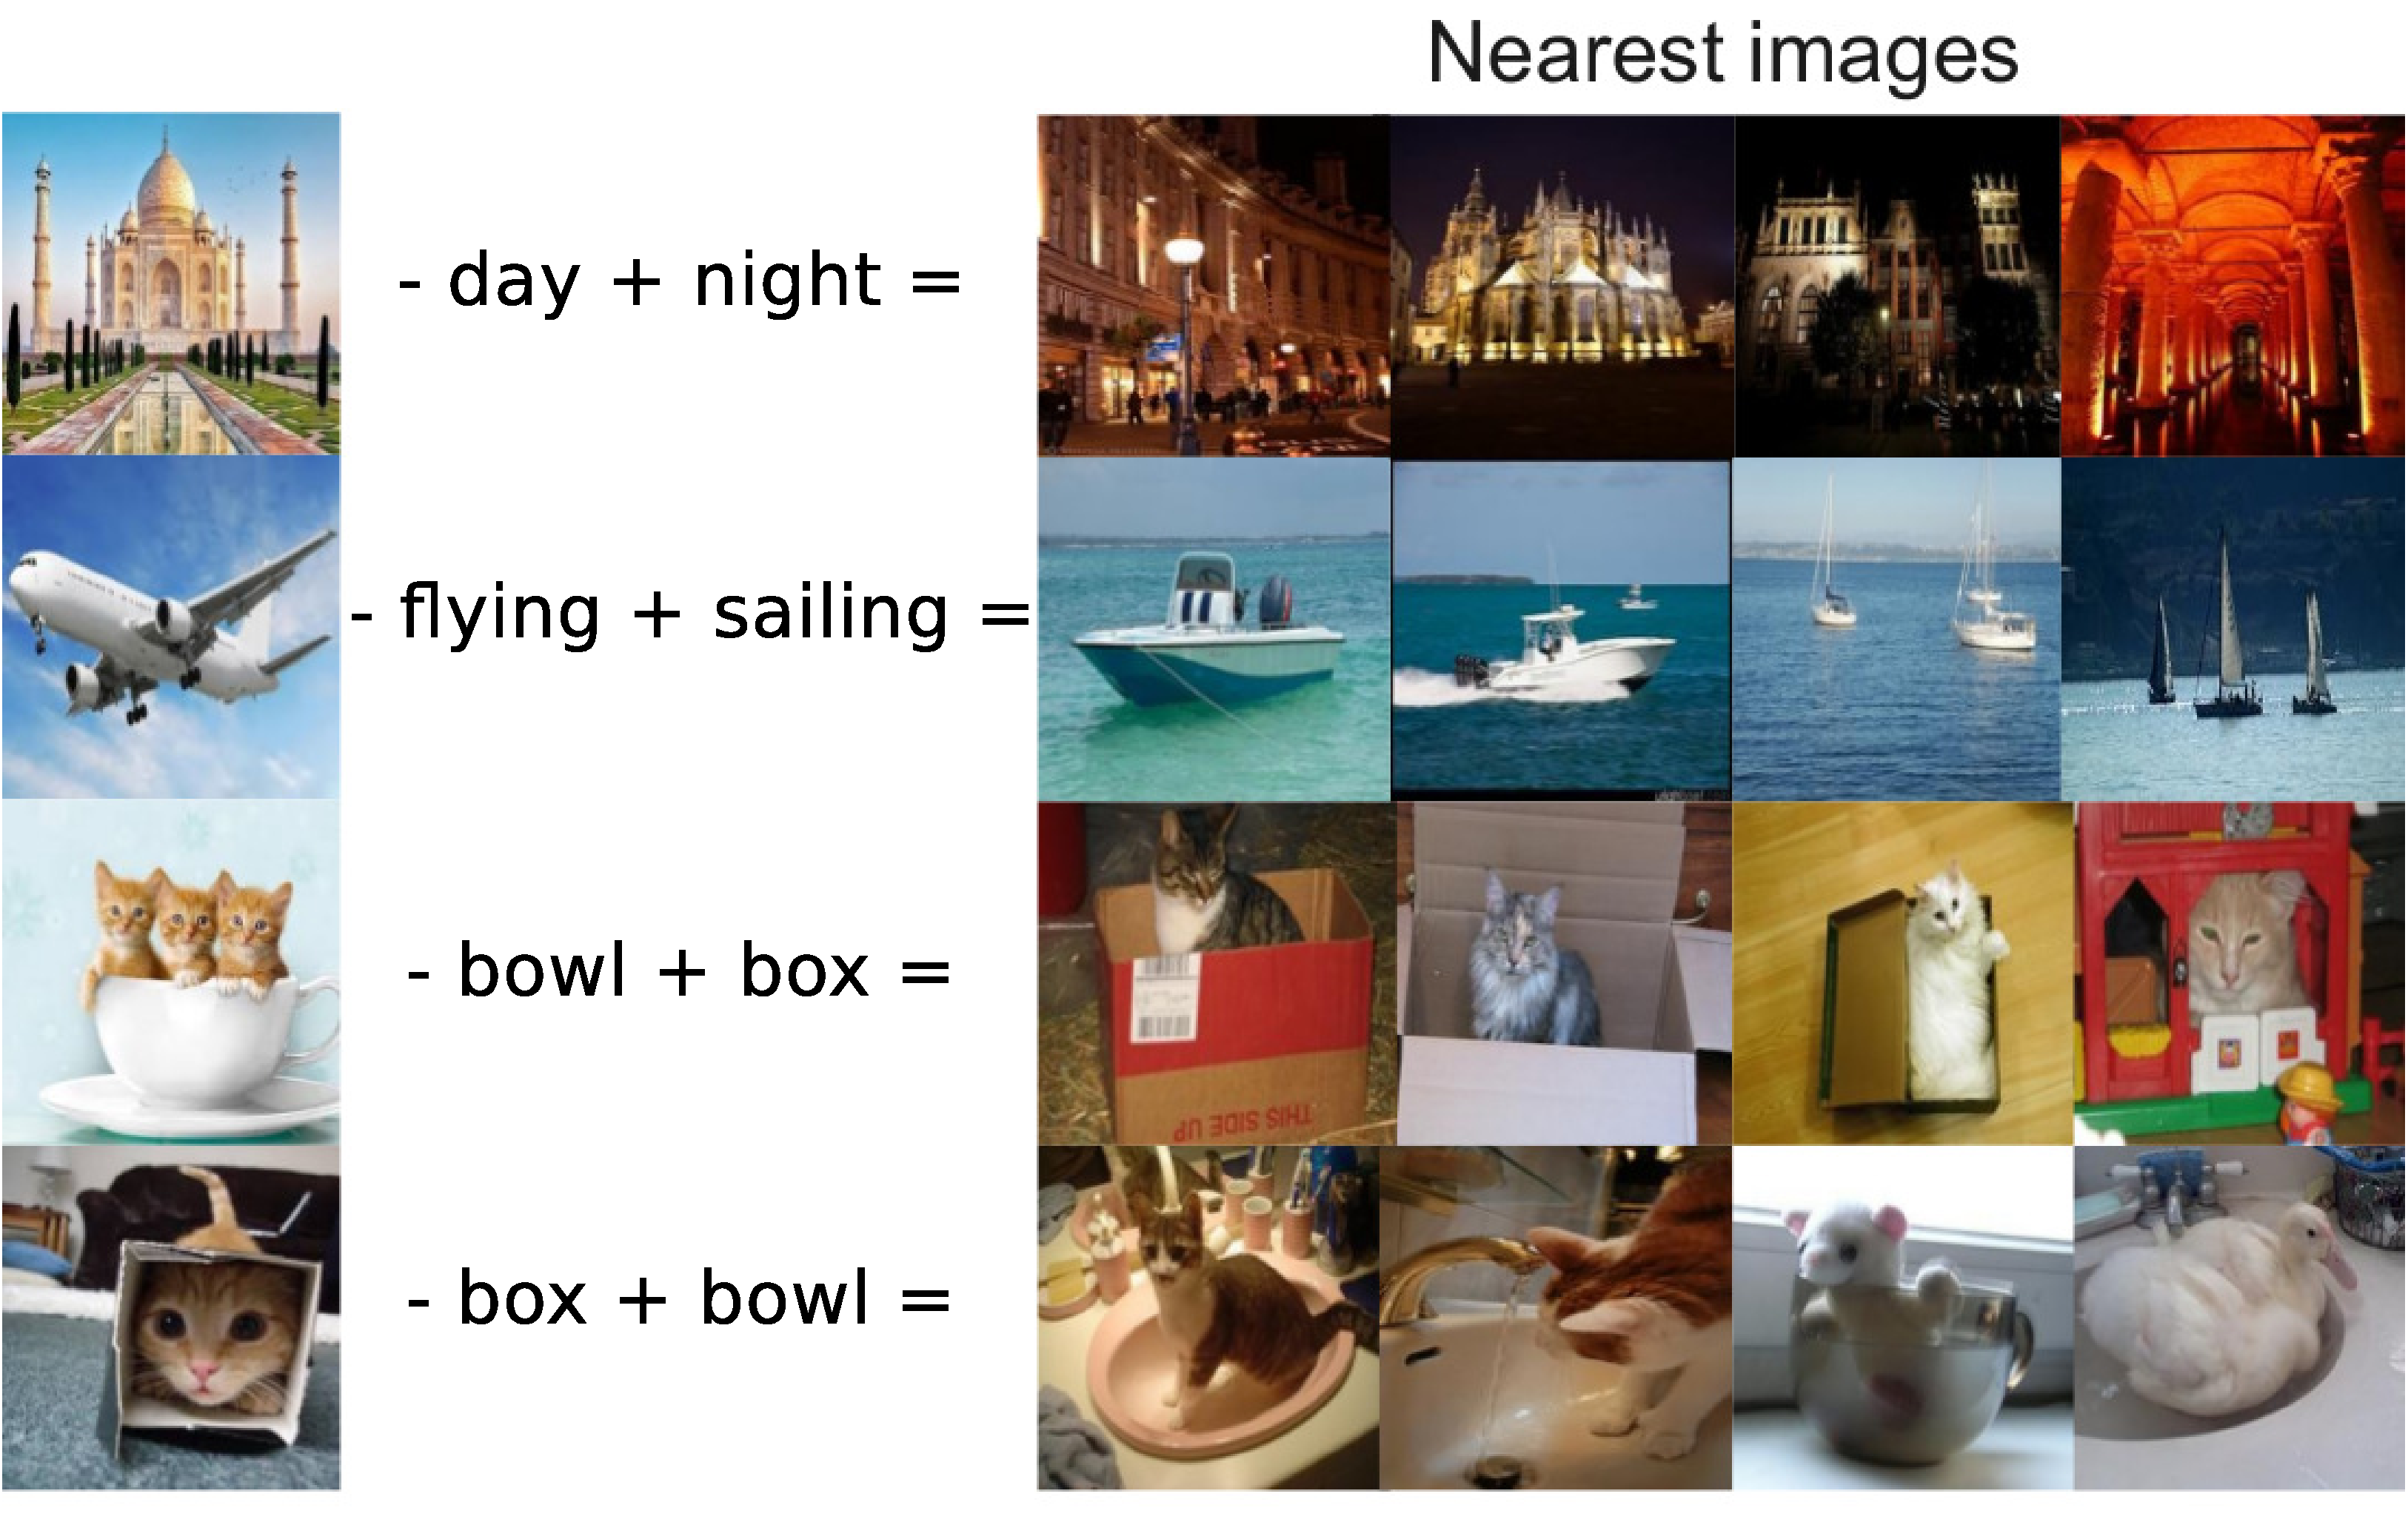
\includegraphics[width=0.33\columnwidth]{others_crop2.pdf}}
      \subfigure[Sanity check]
      {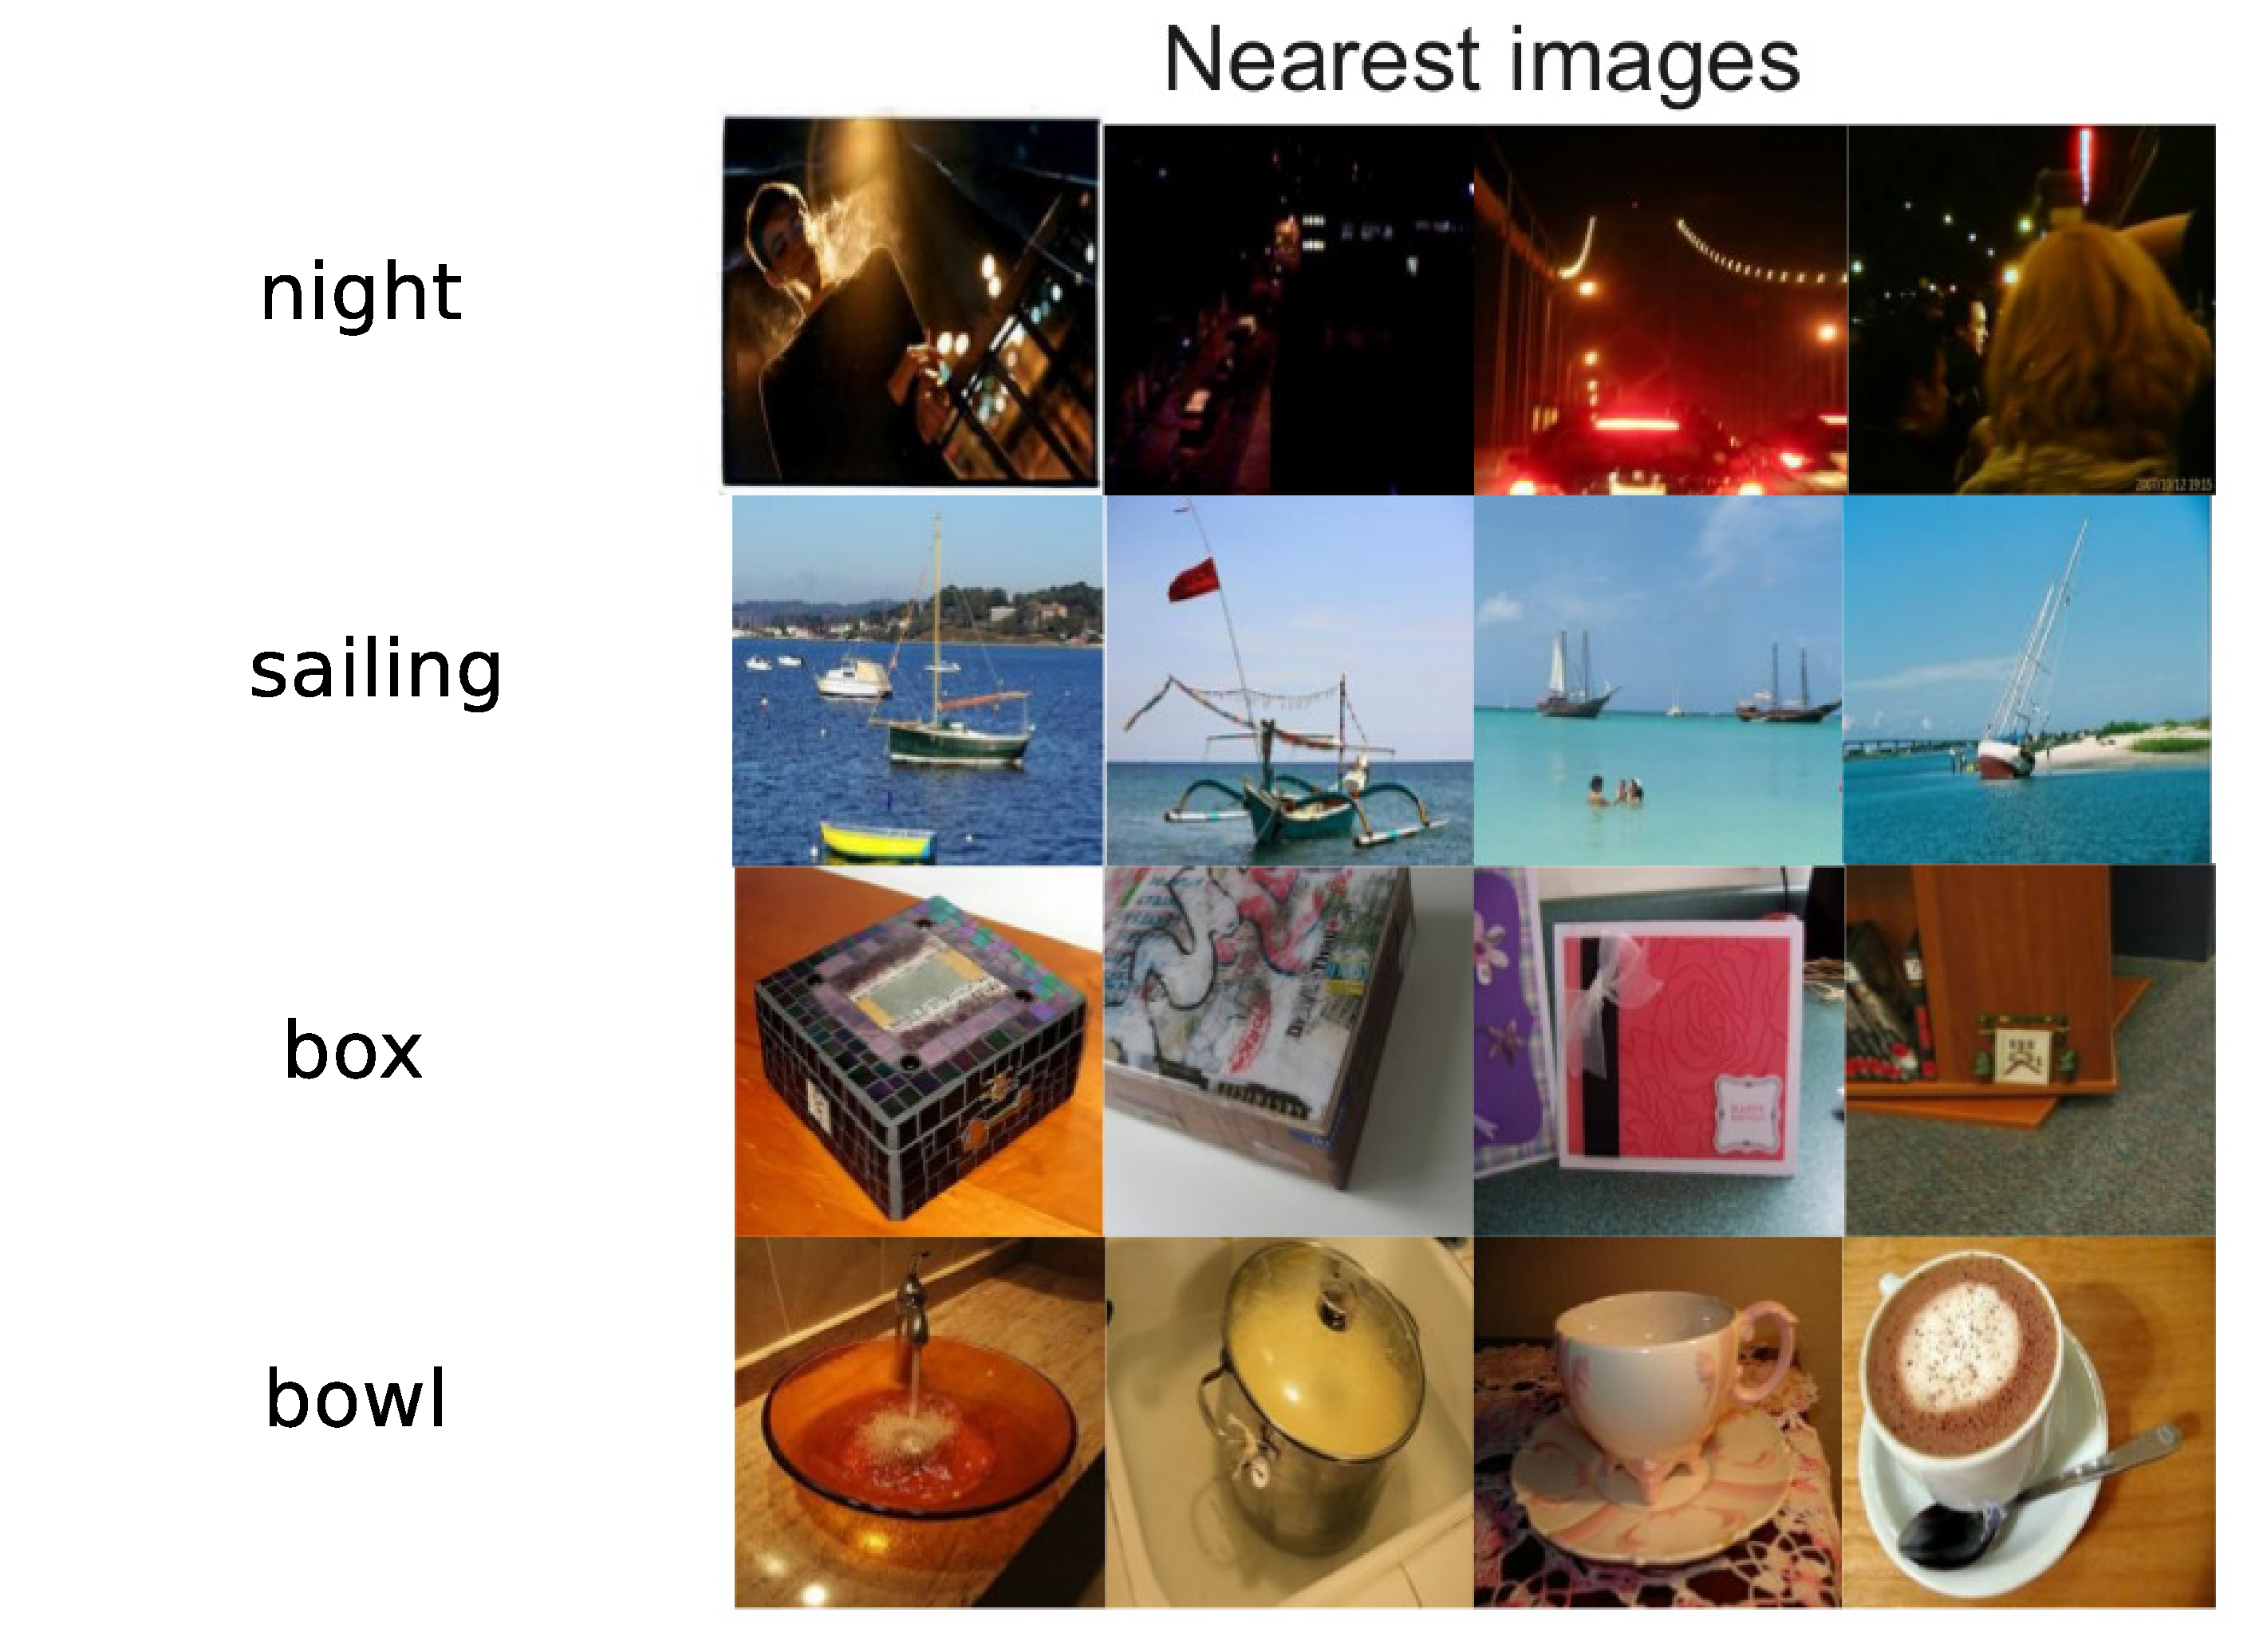
\includegraphics[width=0.285\columnwidth]{sanity_crop2.pdf}}
    }
    \caption{Multimodal vector space arithmetic, for (a) Colors and (b) Image
      structure. The sanity check shows that the retrieved images are not 
      simply the ones associated with the added word.} 
    \label{fig:lr}
  \end{figure}
\end{block}
\vfill
\endminipage
\end{column}%2

%-- Column 3 ---------------------------------------------------
\begin{column}{0.32\linewidth}
\minipage[c][0.9\textheight][s]{\columnwidth}
\vfill

%-- Block 3-4 --------------------------------------------------
\begin{block}{\bf{\large Image-sentence ranking}}
  \begin{itemize}
    \item Image-sentence ranking experiments: Flickr8K and Flickr30K
    \item Image annotation: for each image, rank all descriptions
    \item Image search: for each sentence, rank all images
    \item Retrieval is done within the development/test sets (1000 images)
  \end{itemize}      
  \begin{table}[t]
  \small
  \centering
  \begin{tabulary}{\linewidth}{L|CCCC|CCCC}
    \hline
    \multicolumn{9}{c}{\textbf{Flickr8K}} \\
    \hline
    & \multicolumn{4}{c}{Image Annotation} & \multicolumn{4}{c}{Image Search} \\
    \textbf{Model} & \textbf{R@1} & \textbf{R@5} & \textbf{R@10} & \textbf{Med} \it{r} & \textbf{R@1} & \textbf{R@5} & \textbf{R@10} & \textbf{Med} \it{r} \\
    \hline
    \hline
    Random Ranking & 0.1 & 0.6 & 1.1 & 631 & 0.1 & 0.5 & 1.0 & 500 \\
    \hline
    SDT-RNN \cite{socher2013grounded} & 4.5 & 18.0 & 28.6 & 32 & 6.1 & 18.5 & 29.0 & 29 \\
    $\dagger$ DeViSE \cite{fromedevise2013} & 4.8 & 16.5 & 27.3 & 28 & 5.9 & 20.1 & 29.6 & 29 \\
    $\dagger$ SDT-RNN \cite{socher2013grounded} & 6.0 & 22.7 & 34.0 & 23 & 6.6 & 21.6 & 31.7 & 25 \\
    DeFrag \cite{karpathy2014deep} & 5.9 & 19.2 & 27.3 & 34 & 5.2 & 17.6 & 26.5 & 32 \\
    $\dagger$ DeFrag \cite{karpathy2014deep} & 12.6 & 32.9 & 44.0 & 14 & 9.7 & 29.6 & 42.5 & 15 \\
    m-RNN \cite{mao2014explain} & \textit{14.5} & \textit{37.2} & \textit{48.5} & \textit{11} & 11.5 & \textit{31.0} & 42.4 & 15 \\
    $\dagger$ BRNN \cite{karpathy2014deepvs} & \underline{16.5} & \underline{40.6} & \underline{54.2} & \underline{7.6} & \underline{11.8} & \underline{32.1} & \underline{44.7} & \underline{12.4} \\
    $\ddagger$ NIC (GoogLeNet) \cite{vinyals2014show} & (\textbf{20}) &  & (\textbf{61}) & \textbf{6} & (\textbf{19}) & & (\textbf{64}) & \textbf{5} \\
    \hline
    Our model & 13.5 & 36.2 & 45.7 & 13 & 10.4 & \textit{31.0} & \textit{43.7} & \textit{14} \\
    Our model (OxfordNet) & 18.0 & 40.9 & 55.0 & 8 & 12.5 & 37.0 & 51.5 & 10 \\
    \hline
  \end{tabulary}
  \vspace{-0.05in}
  \label{fig:f8}
  \end{table}    
  \begin{table}[t]
  \small
  \centering
  \begin{tabulary}{\linewidth}{L|CCCC|CCCC}
    \hline
    \multicolumn{9}{c}{\textbf{Flickr30K}} \\
    \hline
    & \multicolumn{4}{c}{Image Annotation} & \multicolumn{4}{c}{Image Search} \\
    \textbf{Model} & \textbf{R@1} & \textbf{R@5} & \textbf{R@10} & \textbf{Med} \it{r} & \textbf{R@1} & \textbf{R@5} & \textbf{R@10} & \textbf{Med} \it{r} \\
    \hline
    \hline
    Random Ranking & 0.1 & 0.6 & 1.1 & 631 & 0.1 & 0.5 & 1.0 & 500 \\
    \hline
    $\dagger$ DeViSE \cite{fromedevise2013} & 4.5 & 18.1 & 29.2 & 26 & 6.7 & 21.9 & 32.7 & 25 \\
    $\dagger$ SDT-RNN \cite{socher2013grounded} & 9.6 & 29.8 & 41.1 & 16 & 8.9 & 29.8 & 41.1 & 16 \\
    $\dagger$ DeFrag \cite{karpathy2014deep} & 14.2 & 37.7 & 51.3 & 10 & 10.2 & 30.8 & 44.2 & 14 \\
    $\dagger$ DeFrag + Finetune CNN & 16.4 & 40.2 & 54.7 & 8 & 10.3 & 31.4 & 44.5 & 13 \\
    m-RNN \cite{mao2014explain} & \textit{18.4} & \textit{40.2} & \textit{50.9} & \textit{10} & 12.6 & 31.2 & 41.5 & 16 \\
    LRCN \cite{donahue2014long} &  &  &  &  & \textit{14.0} & \textit{34.9} & \textit{47.0} & \textit{11} \\
    $\dagger$ BRNN \cite{karpathy2014deepvs} & \underline{22.2} & \underline{48.2} & \underline{61.4} & \textbf{4.8} & \underline{15.2} & \underline{37.7} & \underline{50.5} & \underline{9.2} \\
    $\ddagger$ NIC (GoogLeNet) \cite{vinyals2014show} & (17) &  & (56) & 7 & (\textbf{17}) &  & (\textbf{57}) & \textbf{7} \\
    \hline
    Our model & 14.8 & 39.2 & \textit{50.9} & \textit{10} & 11.8 & 34.0 & 46.3 & 13 \\
    Our model (OxfordNet) & \textbf{23.0} & \textbf{50.7} & \textbf{62.9} & \textbf{5} & \textbf{16.8} & \textbf{42.0} & \textbf{56.5} & 8 \\
    \hline
  \end{tabulary}
  %\vspace{-0.1in}
  \caption{{\small Flickr8K and Flickr30K experiments. \textbf{R@K} is Recall@K
      (high is good). \textbf{Med} {\it r} is the median rank (low is
      good). Best results overall are \textbf{bold}, best results without
      OxfordNet or GoogLeNet features are \underline{underlined} and best
      results that only use single frame features (without OxfordNet or
      GoogLeNet) are \textit{italicized}. A $\dagger$ in front of the method
      indicates that object detections were used along with single frame
      features. A $\ddagger$ indicates that ensembles were used.}} 
  \label{fig:f30}
  \vspace{-0.1in}
  \end{table}
\end{block}    
\vfill

%-- Block 3-5 --------------------------------------------------
\begin{block}{\bf{\large Additional results}}
  \begin{itemize}
  \item \textbf{DEMO:} See deeplearning.cs.toronto.edu/i2t 
  \end{itemize}
\end{block}
\vfill

%-- Block 3-6 --------------------------------------------------
\begin{block}{\bf{\large References}}
  \footnotesize{\bibliography{tacl2014}}
  \footnotesize{\bibliographystyle{unsrt}}
\end{block}

\endminipage
\end{column}%3
\end{columns}
\end{frame}
\end{document}
